\section{Opis problema}

Imamo 49 živil, ki so opisani z 10 parametri in predstavljajo spremenljivke problema, zbrane v vektorju spremenljivk $\Vec{x}$. Vezi med spremenljivkami definiramo ozirajoč se na zdravo prehrano sledeče:
\begin{itemize}
    \item masa vseh živil $\leq$ 2 kg,
    \item maščobe $\geq 70$ g,
    \item ogljikovi hidrati $\geq$ 310 g,
    \item proteini $\geq$ 50 g,
    \item kalcij $\geq$ 1 g,
    \item železo $\geq$ 18 mg,
    \item vitamin C $\geq$ 60 mg,
    \item kalij $\geq$ 3,5 g in
    \item 0,5 $\geq$ natrij $\geq$ 2,4 g.
\end{itemize}

Pri tem se pri obravnavi problema izraz za natrij spremeni v dva pogoja za minimalno in maksimalno vrednost. Tako lahko definiramo poljubno število vezi, ki jih zapišemo v matrični obliki in obvezni pogoj o nenegativnih vrednostih:
$$A \cdot \vec{x} \leq \vec{b} \quad \text{ in } \quad x_i \geq 0 \quad \forall \,i$$

Tako moramo vse vezi, ki nastopajo v obliki $\geq$ pretvoriti v željeno obliko $\leq$, kar se preprosto izpolni z množenjem z -1. Vemo, da je število stolpcev matrike $A$ enako številu spremenljivk (živil), vrednosti, ki nastopajo v njej pa so parametri živil.

Ker želimo minimizirati nekaterega izmed parametrov živil, definiramo cenovno funkcijo da velja 
$$\zeta^T(\vec{x}) \cdot \vec{x} = \text{MIN.}$$

V programskem jeziku \texttt{Python} obstaja rutina za linearno programiranje \linebreak \texttt{scipy.optimize.linprog}, ki sprejema vezi oblike $\leq$, pogoj o nenegativnih vrednostih pa je že privzeto izpolnjen.

\section{Minimalna količina kalorij}

Ob zgornjih vezeh minimiziramo kalorije tako, da za cenovno funkcijo izberemo

$$\zeta(cena) = \sum_j cena_j \, x_j = \text{MIN}$$

Po rešitvi dobimo presenetljive rezultate, prikazane na sliki \ref{fig:min_kalorije} in preglednici \ref{tab:min_kalorije}, saj lahko zadostimo vezem,ko več kot polovico zaužitega predstavlja Radenska, pijače skupaj pa celo 89,4 \%. Pri tem \textbf{skupna energijska vrednost živil znaša 1297 kcal}. V prehrani je v tem primeru uporabljenih le 12 \% od vseh živil na izbiro.
\begin{figure}[ht!]
    \centering
    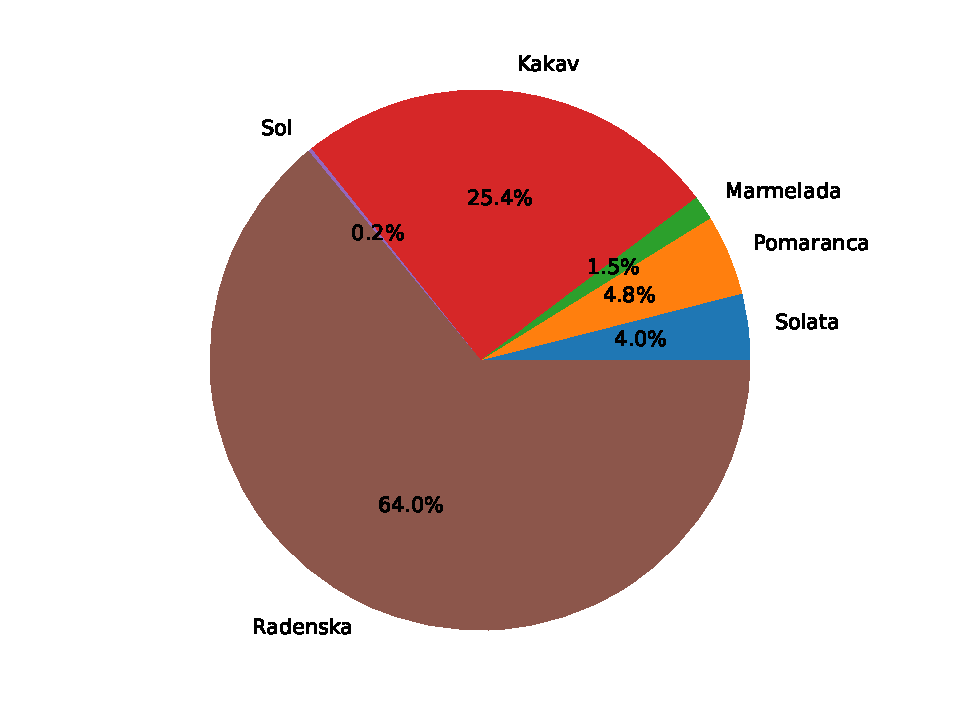
\includegraphics[width=0.85 \textwidth]{2.nal_slike/1.primer.pdf}
    \caption{Rezultat masnih deležev prisotnih živil ob minimizaciji kalorij.}
    \label{fig:min_kalorije}
\end{figure}
\begin{table}[H]
    \centering
    \begin{tabular}{|c|c|c|}
    \hline
    živilo & masa [g] & energija [kcal] \\
    \hline
    Radenska & 1280 & 0 \\
    \hline
    Kakav & 508 & 1165 \\
    \hline
    Pomaranča & 96 & 45 \\
    \hline
    Solata & 79 & 14 \\
    \hline
    Marmelada & 29 & 73 \\
    \hline
    Sol & 4 & 0 \\
    \hline
    $\sum$ & 2000 & 1297 \\
    \hline
    \end{tabular}
    \caption{Količina in minimizirana vrednost prisotnih živil pri minimizaciji kalorij.}
    \label{tab:min_kalorije}
\end{table}
\begin{figure}[H]
    \centering
    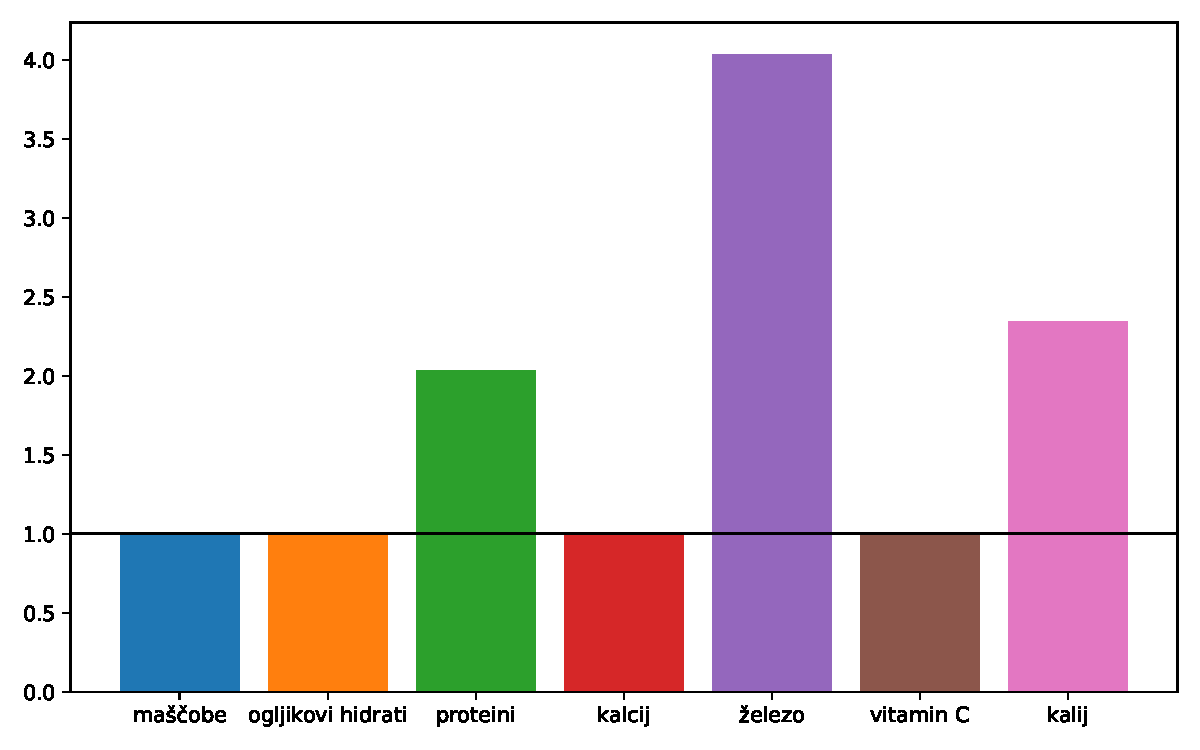
\includegraphics[width=\textwidth]{2.nal_slike/1.primer_vezi.pdf}
    \caption{Razmerje doseženih parametrov z minimalnimi, zahtevanimi v vezeh za primer minimizacije energije.}
    \label{fig:rez_vezi_1}
\end{figure}

\section{Minimalen vnos maščob}

Pri tem uvedemo novo vez
\begin{center}
    kalorije $\geq$ 2000 kcal
\end{center}
in ob tem minimiziramo maščobe po cenovni funkciji $$\zeta(\textit{maščobe}) = \sum_j \textit{maščobe}_j \, x_j = \text{MIN}$$

V tem primeru znaša \textbf{minimizirana količina maščob 70 g}, kar je pričakovano, saj je to minimalni pogoj, zahtevan v vezeh. Ponovno je zelo malo uporabljenih živil, le 10 \%. Vrednosti preostalih parametrov so vidni na sliki \ref{fig:2.vezi}.

\begin{figure}[ht!]
    \centering
    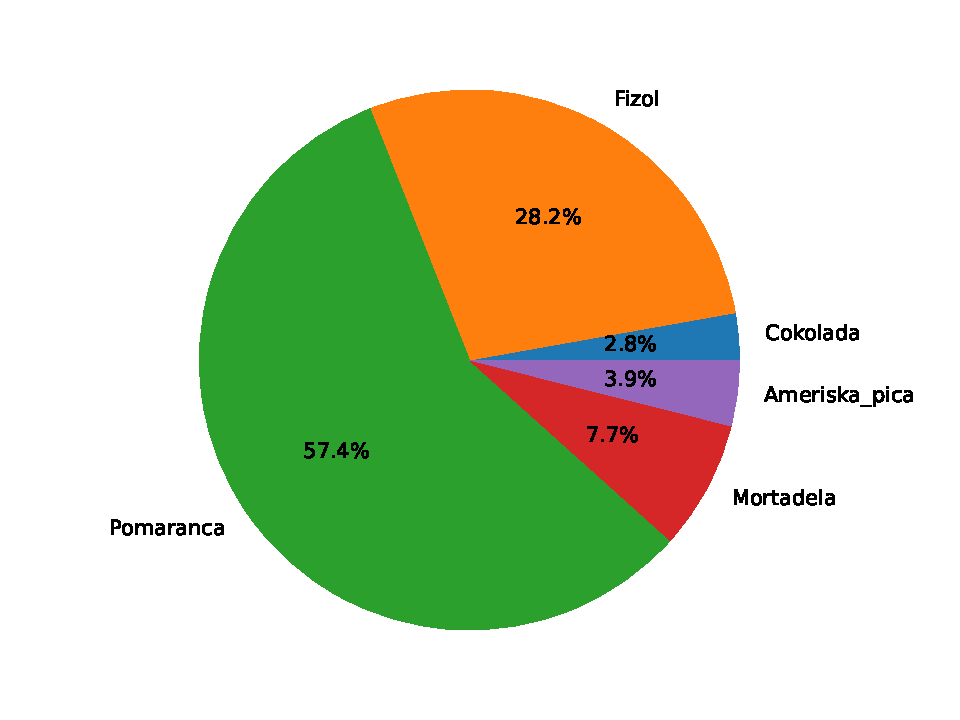
\includegraphics[width= 0.85 \textwidth]{2.nal_slike/2.primer.pdf}
    \caption{Rezultat masnih deležev prisotnih živil ob minimizaciji maščob.}
    \label{fig:min_maščobe}
\end{figure}
\begin{table}[H]
    \centering
    \begin{tabular}{|c|c|c|}
    \hline
    živilo & masa [g] & maščobe [g] \\
    \hline
    Pomaranča & 1147 & 1 \\
    \hline
    Fižol & 563 & 3 \\
    \hline
    Mortadela & 154 & 39 \\
    \hline
    Ameriška pica & 78 & 8 \\
    \hline
    Čokolada & 56 & 19 \\
    \hline
    $\sum$ & 2000 & 70 \\
    \hline
    \end{tabular}
    \caption{Količina in minimizirana vrednost prisotnih živil pri minimizaciji maščob.}
    \label{tab:min_maščobe}
\end{table}
\begin{figure}[H]
    \centering
    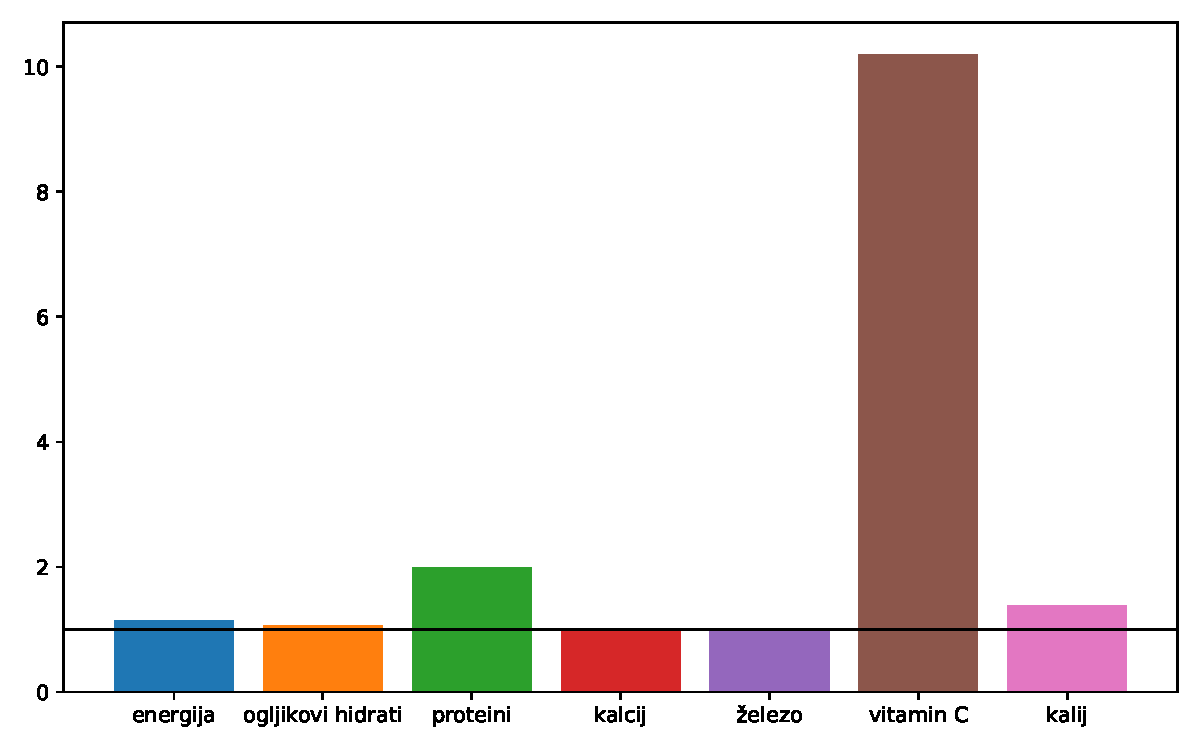
\includegraphics[width=\textwidth]{2.nal_slike/2.primer_vezi.pdf}
    \caption{Razmerje doseženih parametrov z minimalnimi, zahtevanimi v vezeh za primer minimizacije maščob.}
    \label{fig:2.vezi}
\end{figure}

\section{Minimalna cena}

Ob prejšnjih vezeh definiramo novo cenovno funkcijo $$\zeta(\textit{cena}) = \sum_j \textit{cena}_j \, x_j = \text{MIN}$$ po kateri minimiziramo ceno in dobimo najcenejši dnevni vnos hrane \textbf{z ceno 1,43 evrov}. 
\begin{figure}[H]
    \centering
    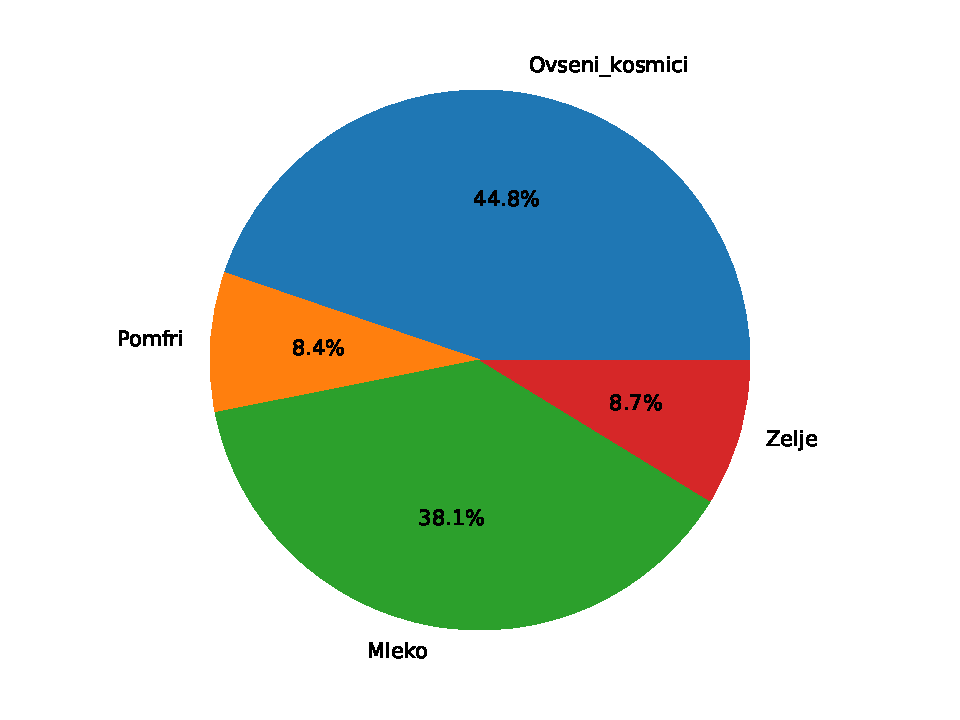
\includegraphics[width= 0.85 \textwidth]{2.nal_slike/3.primer.pdf}
    \caption{Rezultat masnih deležev prisotnih živil ob minimizaciji cene.}
    \label{fig:min_cena}
\end{figure}
\begin{table}[H]
    \centering
    \begin{tabular}{|c|c|c|}
    \hline
    živilo & masa [g] & cena [EUR] \\
    \hline
    Ovseni kosmiči & 628 & 0,69 \\
    \hline
    Mleko & 535 & 0,54 \\
    \hline
    Zelje & 122 & 0,09 \\
    \hline
    Pomfri & 117 & 0,11 \\
    \hline
    $\sum$ & 1405 & 1,43 \\
    \hline
    \end{tabular}
    \caption{Količina in minimizirana vrednost prisotnih živil pri minimizaciji cene.}
    \label{tab:min_maščobe}
\end{table}
\begin{figure}[H]
    \centering
    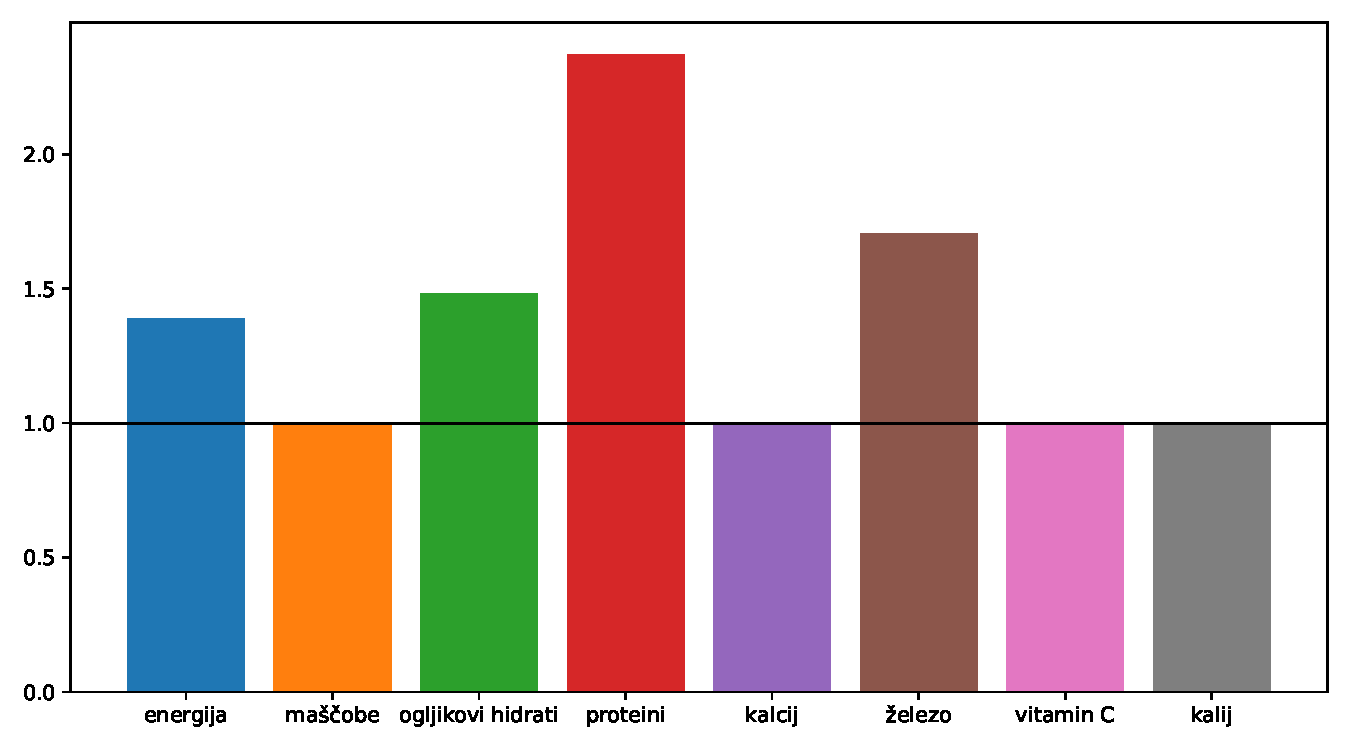
\includegraphics[width=\textwidth]{2.nal_slike/3.primer_vezi.pdf}
    \caption{Razmerje doseženih parametrov z minimalnimi, zahtevanimi v vezeh za primer minimizacije cene.}
    \label{fig:3.vezi}
\end{figure}

\section{Omejitev količine živil}

Ker prehrana v zgornjih primerih ni raznovrstna, saj zaužijemo le okoli 10 \% od vseh živil na voljo, želimo povečati pestrost prehrane. Verjetno najenostavnejša možnost je, da omejimo največjo dovoljeno količino zaužitega živila, saj se to enostavno sprogramira kot vhodni podatek za rutino \texttt{scipy.optimize.linprog}. Tako nastane ‘prostor’ za nova živila v prehrani, vendar se zato zviša optimalna minimalna vrednost izračunana brez tega dodatnega pogoja.

\begin{figure}[ht!]
    \centering
    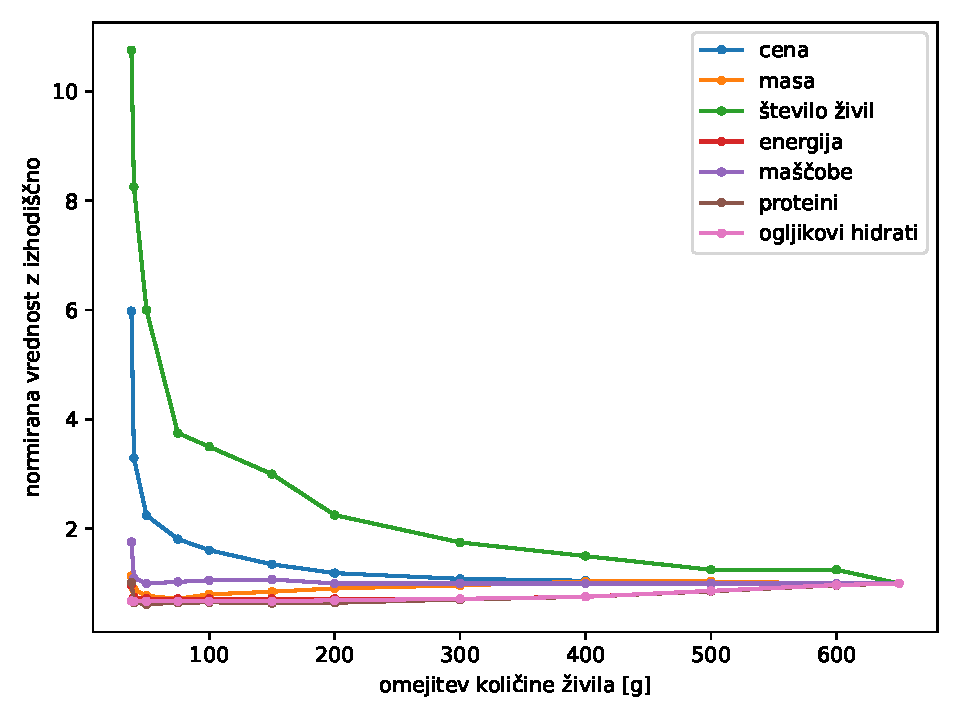
\includegraphics[width=\textwidth]{2.nal_slike/vpliv_omejitve_zivil.pdf}
    \caption{Razmerje med izračunanimi parametri ob omejitvi števil in onimi brez omejitve ob minimizaciji cene.}
    \label{fig:vpliv_omejitve}
\end{figure}

Opazimo, da število živil narašča z zmanjševanjem omejitve, prav tako minimizirana vrednost, medtem ko ostale padajo, glede na začetno stanje, vendar se gibljejo blizu minimalnih, zahtevanih v vezeh. Z zmanjševanjem omejitve se veča količina preostalih živil pod omejitvenim pragom, vendar med njimi in novimi živili ni moč povezave najti. Porast vseh vrednosti pri najmanjši omejitvi si lahko razlagamo, kot da zaradi premajhne izbire živil ni več moč tako dobro izbrati parametrov.

\newpage
\section{Omejitev vnosa tekočine}

Zanimive rezultate dobimo, če uvedemo dodaten parameter -- VODO -- in v vezeh zahtevamo, da jo zaužijemo vsaj 1 l. Pri tem smo upoštevali, da je voda prisotna le v pijačah, kot je dopolnjeno v datoteki \texttt{tabela-zivil.dat}. Ob minimizaciji maščob in brez pogoja o omejitvi posameznega živila dobimo precej neuravnovešena živila, ob vpeljavi pogoja za vodo pa dobimo bolj realen približek prehrane.

\begin{figure}[ht!]
\begin{centering}
    \begin{subfigure}[b]{.48\textwidth}
        \centering 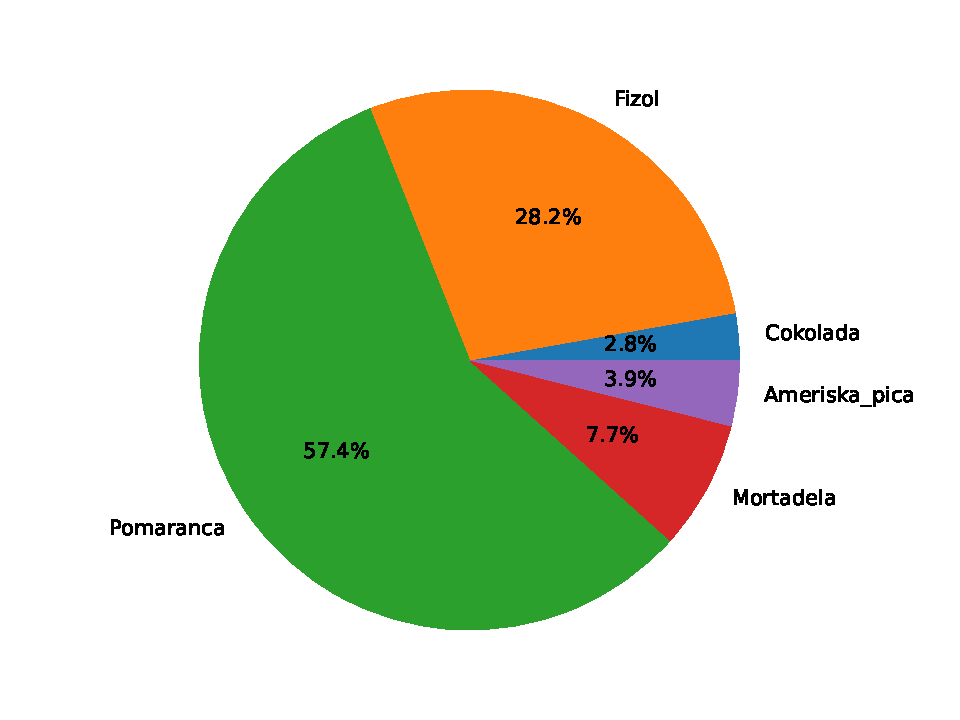
\includegraphics[scale=0.5]{2.nal_slike/brez_vez_vode.pdf}
    \end{subfigure}
    \quad
    \begin{subfigure}[b]{.48\textwidth}
        \centering 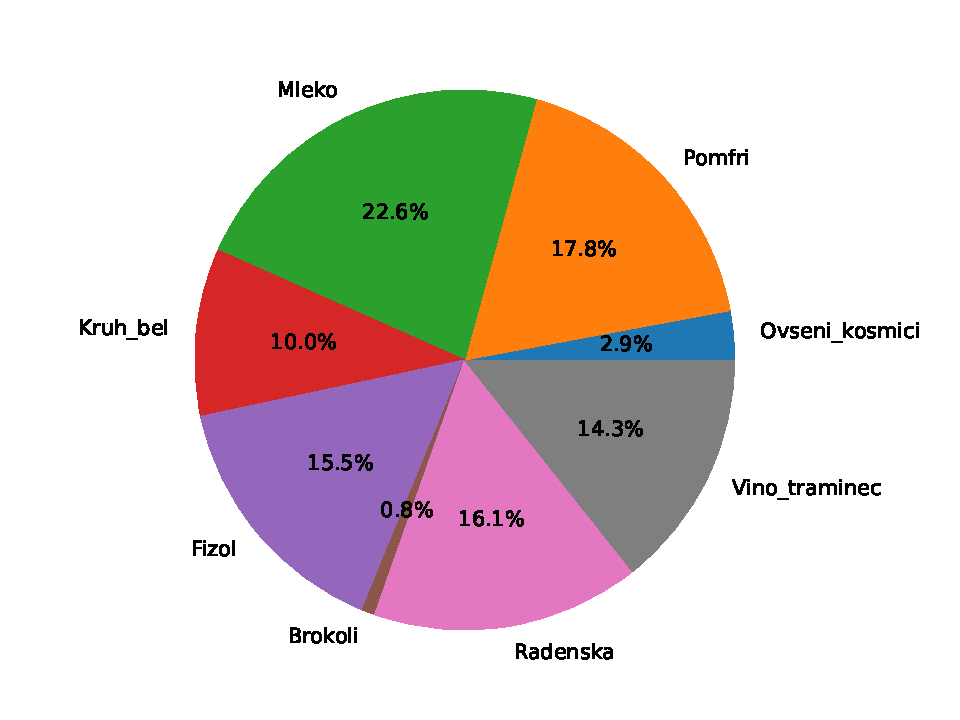
\includegraphics[scale=0.5]{2.nal_slike/vez_vode.pdf}
    \end{subfigure}
    \quad
    \caption{Vpliv pogoja za vodo na rezultate ob minimizaciji maščob: levo brez, desno z pogojem.}
    \label{fig:vpliv_vode}
\end{centering}
\end{figure}